\documentclass{beamer}
\usetheme{Madrid}

\usepackage{amsmath, amssymb, amsthm}
\usepackage{graphicx}
\usepackage{listings}
\usepackage{gensymb}
\usepackage[utf8]{inputenc}
\usepackage{hyperref}
\usepackage{gvv}

\begin{document}

\title{Gate 2022 NM}
\author{EE23BTECH11016 - Aditi Dure$^{*}$}
\date{}
\frame{\titlepage}

\begin{frame}
\frametitle{Question 40}
%content
Consider the wave elevation spectrum $S_{\eta \eta}(\omega)$ as shown in the figure. Then, the significant wave height is \underline{\hspace{3cm}} m. \\
\hfill{GATE NM 2022}
\end{frame}

\begin{frame}
\frametitle{Plot Given In Question}
\begin{figure}[H]
    \centering
    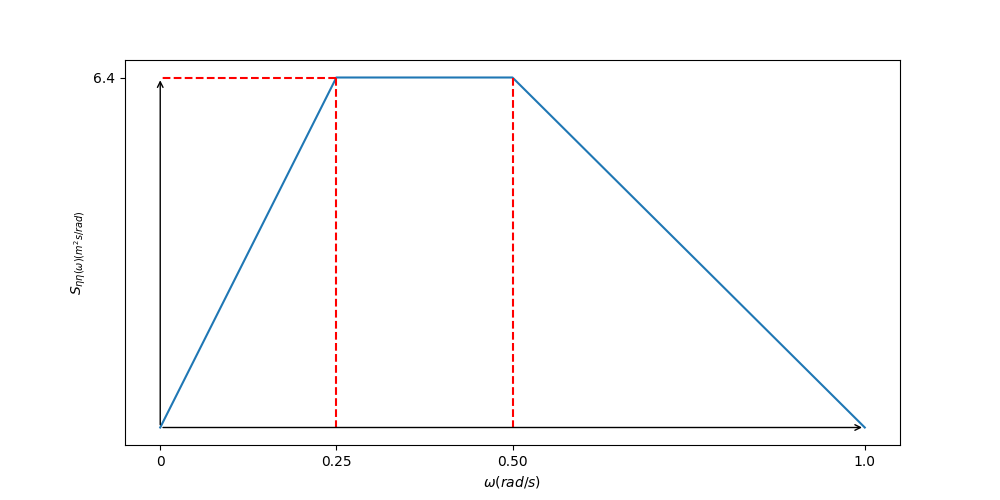
\includegraphics[width=\columnwidth]{./figs/qfig.png}
    \caption{Wave Elevation Spectrum}
    \label{fig: GATE22NM40.1}
\end{figure}
\end{frame}

\begin{frame}
\frametitle{Options}
\begin{enumerate}
\item 2
\item 4
\item 6
\item 8
\end{enumerate}
\end{frame}

\begin{frame}
\frametitle{Solution}
Given:
\begin{align}
S_{\eta \eta}(\omega)(m^2s/rad) = 
\begin{cases}
  25.6\omega   & \text{if } \omega \in [0,0.25] \\
  6.4  & \text{if } \omega \in (0.25,0.50] \\
  12.8\omega-12.8  & \text{if } \omega \in (0.50,1.0] \\
  0  & o.w \\
\end{cases}
\end{align}
\end{frame}

\begin{frame}
\frametitle{Solution}
In terms of f:
\begin{align}
S_{\eta \eta}(f)(m^2s) = 
\begin{cases}
  51.2\pi f   & \text{if } f \in [0,\frac{\pi}{2}] \\
  6.4  & \text{if } f \in (\frac{\pi}{2},\pi] \\
  25.6\pi f-12.8  & \text{if } f \in (\pi,2\pi] \\
  0 & o.w \\
\end{cases} \label{eq: GATE22NM40.1}
\end{align}
\end{frame}

\begin{frame}
\frametitle{Solution}
Significant Wave Height:
\begin{align}
H_s &= 4 \sqrt{\int_{0}^{\infty} S(f)df}
\end{align}
\end{frame}

\begin{frame}
\frametitle{Solution}
From \eqref{eq: GATE22NM40.1}
\begin{align}
H_s &= 4 \sqrt{\int_{0}^{\frac{\pi}{2}} 51.2\pi fdf + \int_{\frac{\pi}{2}}^{\pi} 6.4df + \int_{\pi}^{2\pi} (25.6\pi f-12.8)df} \\
&= 4 \sqrt{0.8 +1.6 +1.6} \\
\therefore H_s &= 8
\end{align}
Hence the answer is option (D).
\end{frame}

\end{document}
